\documentclass[10pt, scrartlc]{article}
%\documentclass{article}
\usepackage[font={sf}]{caption}
\usepackage[]{graphics}
\usepackage{graphicx}
\usepackage{epstopdf}
\usepackage{hyperref}
\hypersetup{breaklinks=true, colorlinks=true, citecolor=blue}
\usepackage{natbib}
\usepackage{color}
\usepackage{soul}
\usepackage{rotating}
\usepackage{tabularx}
\usepackage{longtable}
\usepackage{lscape}
\usepackage{array}
\usepackage{multirow}
\usepackage{setspace}
\usepackage{textcomp}
\usepackage{dcolumn}
\setlength{\LTcapwidth}{6in}
\usepackage{dcolumn}
\usepackage[margin=1in]{geometry}
\usepackage{tocloft}
\usepackage{caption}

 \bibpunct{(}{)}{,}{a}{}{,}
 \doublespacing
 \raggedright
 \setlength{\parindent}{15pt} 


\begin{document}

\pagecolor{white}

\begin{center}
{ \Large \bf Figures }
\end{center}

\listoffigures

\clearpage
\newpage

\begin{figure}[h]
	\begin{center}
		\includegraphics[width = 6.5in]{Fig1_ConceptFig.pdf}
	\end{center}
	\caption[Genomic Basis of Local Adaptation Regions]{Description of five conceptual regions that correspond to different genomic architectures that underlie trait divergence across our parameter space (A-B). Each region corresponds to what occurred in both with-inversion simulations (B with-inversion mutation column) and paired no-inversion control simulations (B no-inversion mutation column). Manhattan plot examples are provided for four regions with no-inversion control example on top and with-inversion simulation on the bottom (C). Alternating light and dark blue represent different linkage groups, grey square points represent the neutrally evolving linkage group, and tanbars represent locally adaptive inversions present in the population. }
\end{figure}

\clearpage
\newpage

\begin{figure}[h]
	\begin{center}
		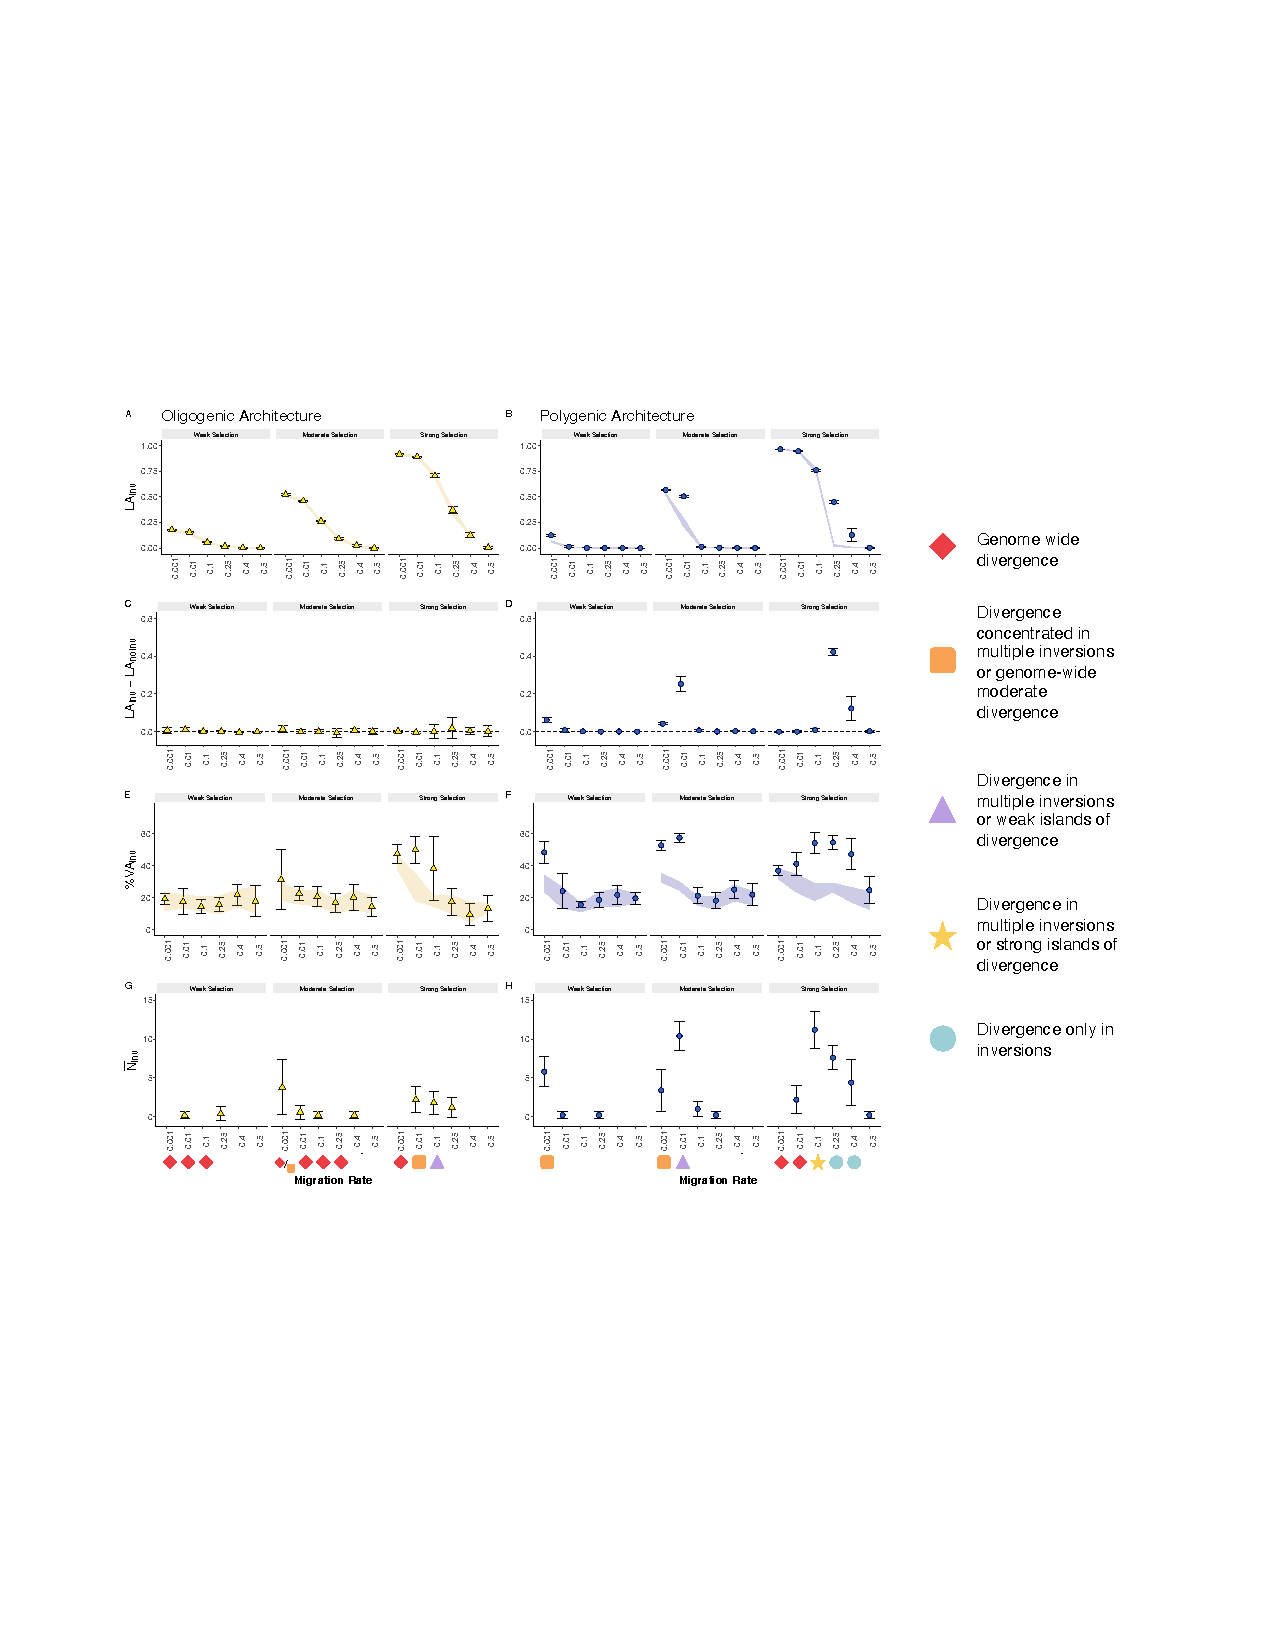
\includegraphics[width = 6.5 in]{Fig2_LA.pdf}
	\end{center}
	\caption[Local Adaptation]{The average amount of local adaptation that is reached in simulations that include inversions plotted as a function of migration rate and split between three panels representing weak, moderate and strong selection for the A) oligogenic and B) polygenic architectures. The ribbon represents one standard deviation for the average local adaptation expected under the null which is the paired no-inversion control simulations. The difference between the average local adaptation reached in with-inversion simulations and paired no-inversion control simulation is shown for the C) oligogenic and D) polygenic architectures. The percent of additive genetic variance found inside inverted regions is plotted for the E) oligogenic and F) polygenic architectures. The ribbon represents one standard deviation for the average percent of the genome that is inverted. The average number of adaptive inversions is plotted for the G) oligogenic and H) polygenic architectures. All averages are across five replicate simulations and all error bars represent one standard deviation. Region symbols for simulations with local adaptation are plotted at the bottom of the figure with a brief description of the region?s genomic architecture for both with-inversion and no-inversion control simulations. All results are shown for simulations that included environmental variance.}
\end{figure}

\clearpage
\newpage

\begin{figure}[h]
	\begin{center}
		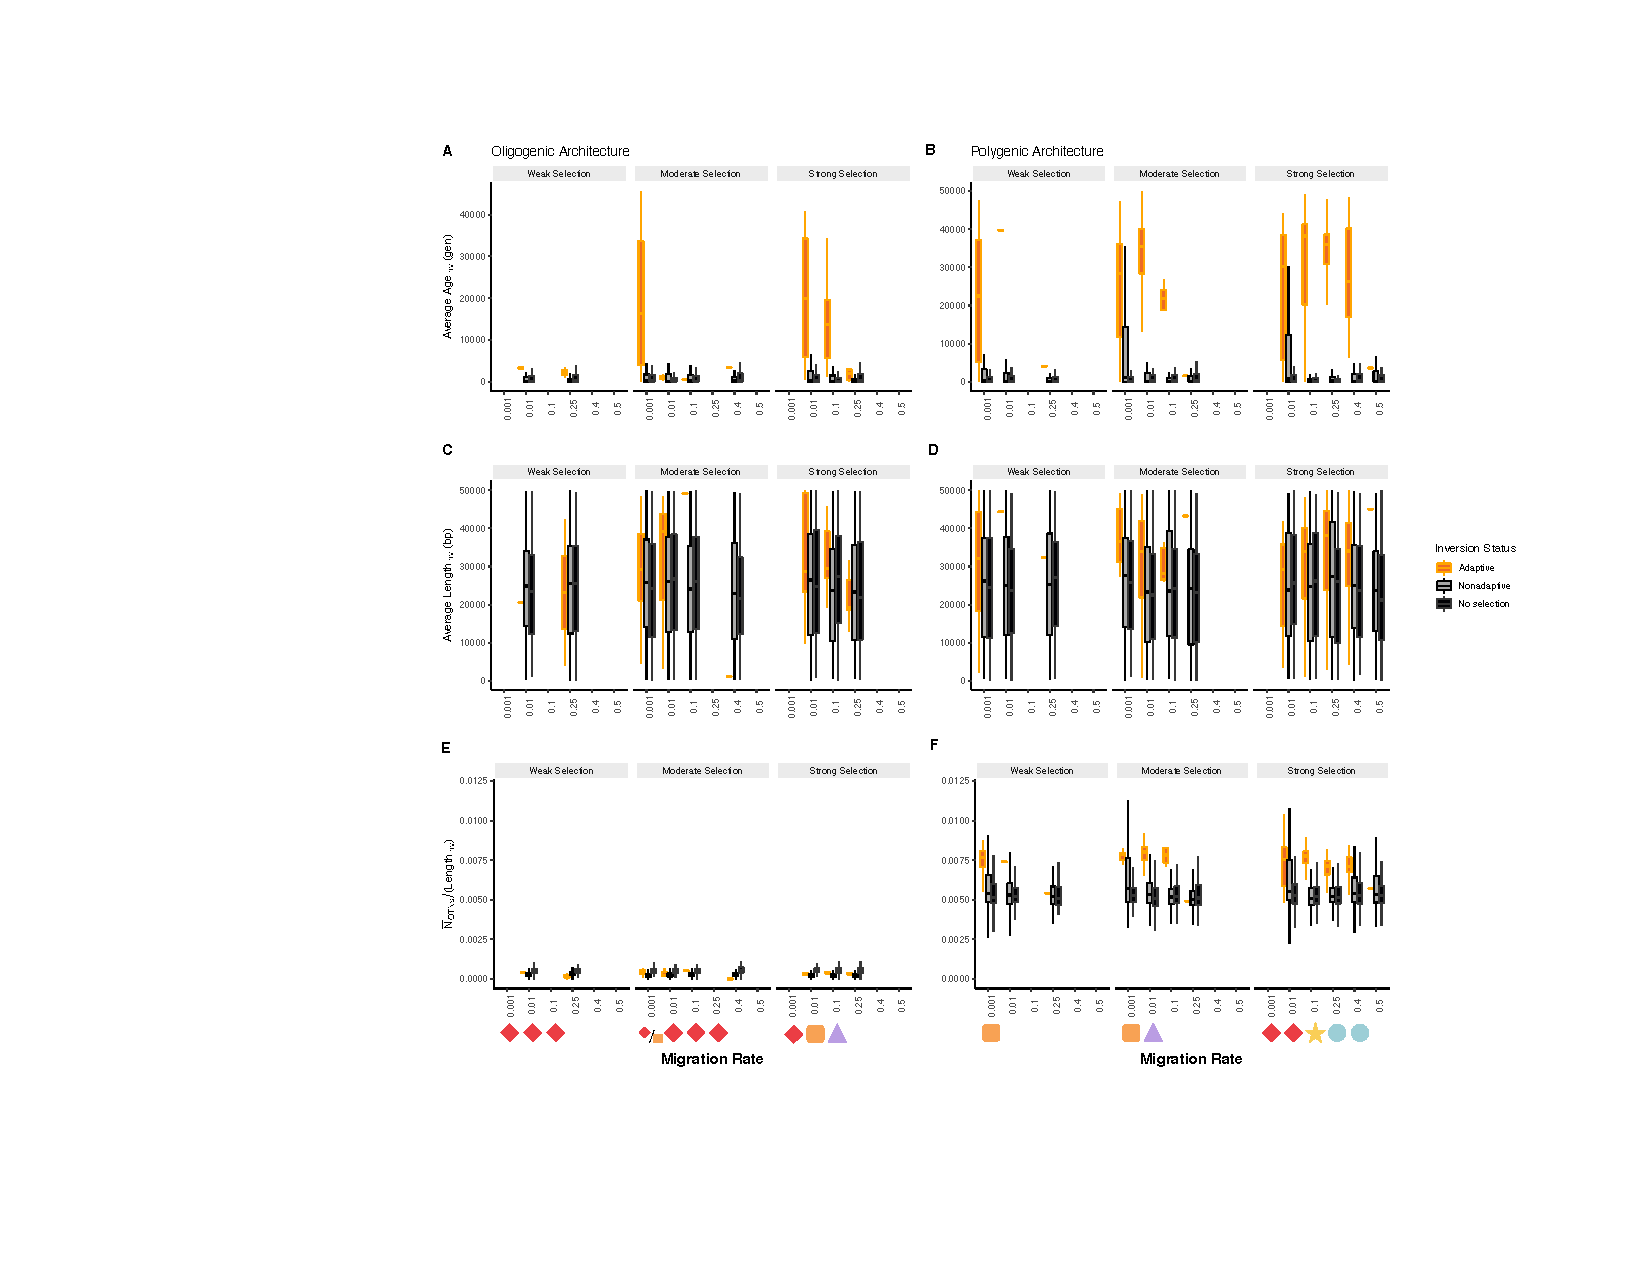
\includegraphics[width = 6.5 in]{Fig3_characteristics.pdf}
	\end{center}
	\caption[Inversion Characteristics]{The average across all simulations of three inversion characteristics, A)  inversion age in generations (gen), B)  inversion length in base pairs (bp), average number of inversion quantitative trait nucleotides (QTNs) scaled by the total length of the inversion for C) oligogenic and D) polygenic architectures. Adaptive inversions are plotted in orange, nonadaptive inversions in light grey, and inversions from the no-selection control simulation in black.
 All results are shown for simulations that included environmental variance.}
\end{figure}

\clearpage
\newpage


\begin{figure}[h]
	\begin{center}
		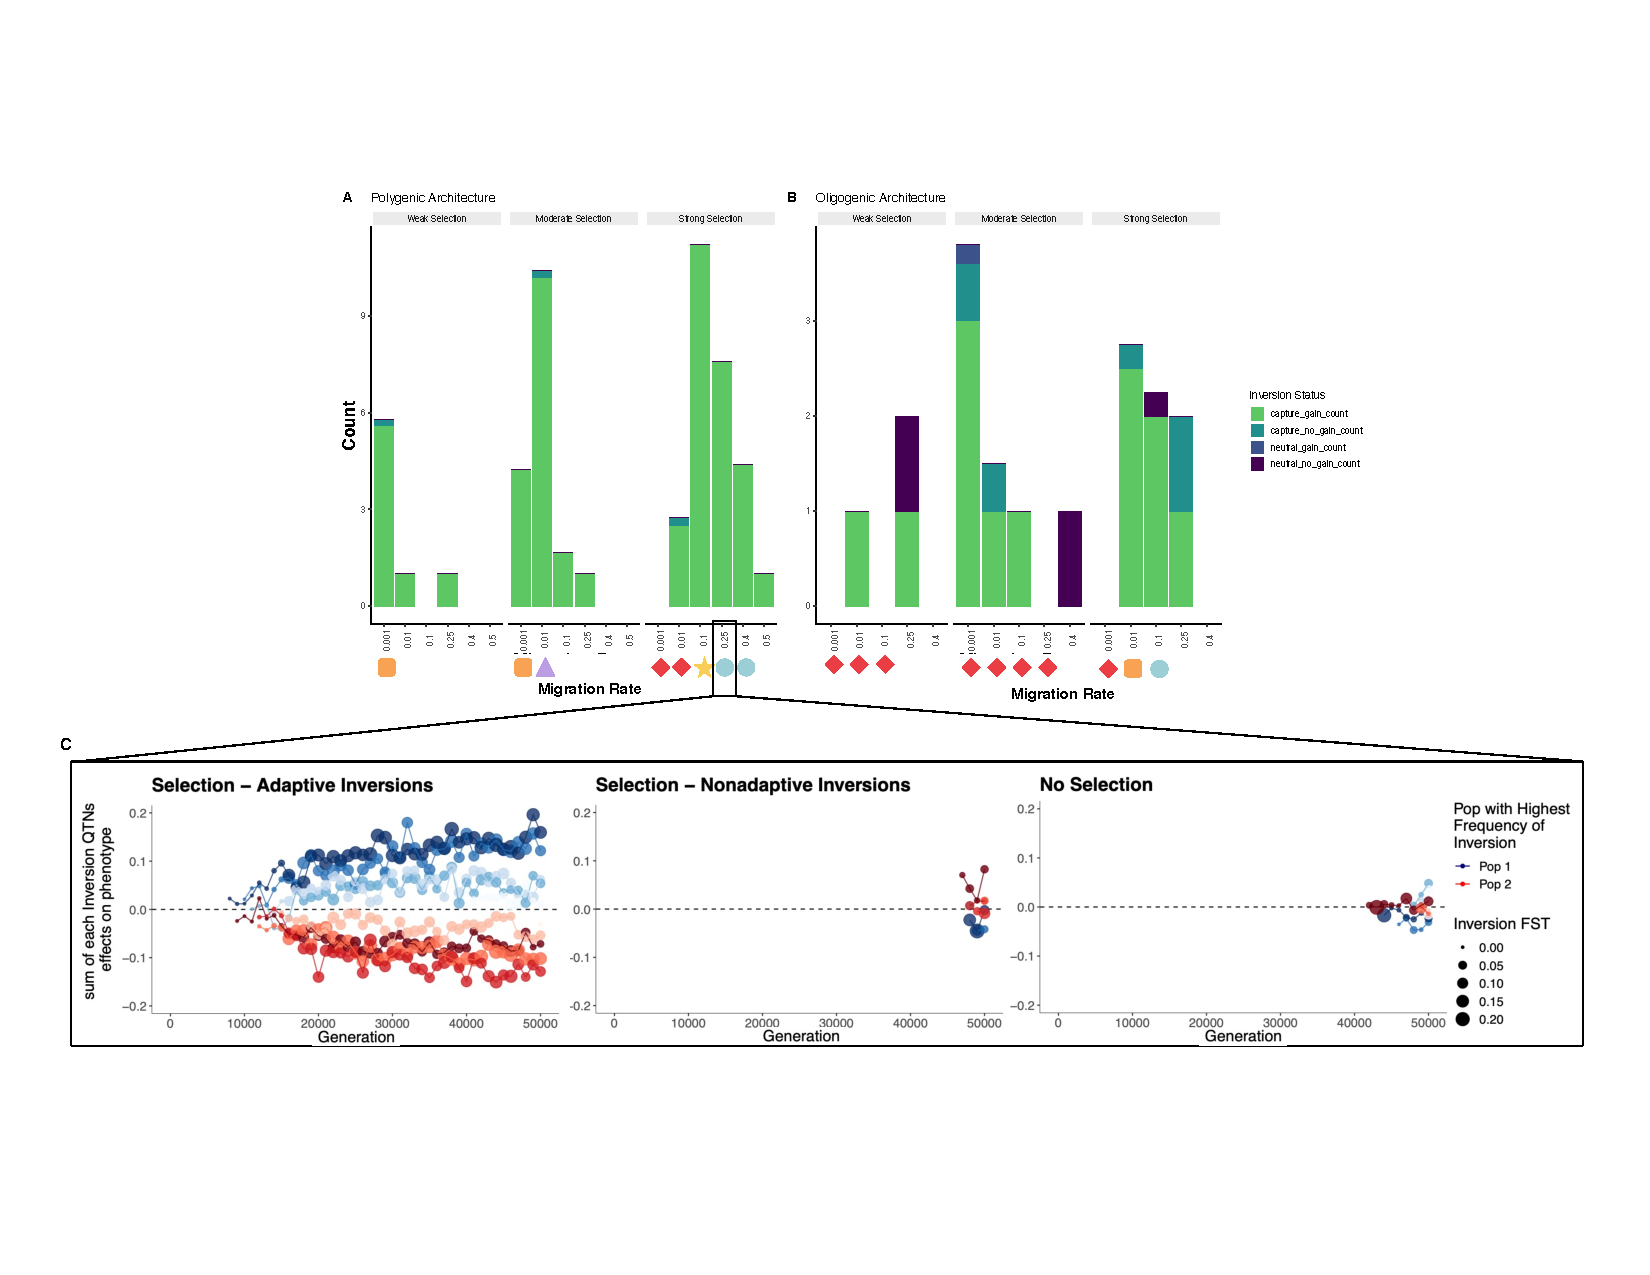
\includegraphics[width = 6.5 in]{Fig4_evoHist.pdf}
	\end{center}
	\caption[Evolutionary History of Adaptive Inversions]{The average number of adaptive inversions (across five replicate simulations) belonging to each of three possible categories: capture then gain (light green), capture then no gain, and neutral then gain (A left panel). An example of the dynamics of the capture and gain category is plotted as the sum of inversion effect size on the phenotype plotted through time for a simulation where inversions facilitated adaptation for adaptive inversions (A right panel). Each track line is an inversion and colors represent which population the inversion is segregating in with blues being population 1 and reds being populating 2 with individuals evolving to \+1 or \-1 phenotype, respectively. Point size is the F\textsubscript{ST} value for the inversion at each time step. Dynamics are also plotted for the paired nonadaptive inversions (B left panel) and no-selection control simulations (B right panel).}
\end{figure}


\end{document}